\chapter{Analisis}
Pada bagian ini, masalah akan dianalisi lebih lanjut. Awalnya, masalah akan dimodelkan terlebih dahulu. Hasil dari pemodelan masalah akan digunakan untuk membentuk masalah \textit{linear program} yang akan diselesaikan menggunakan teknik \textit{linear programming}. Dengan menggunakan \textit{linear programming}, solusi optimal bagi masalah dapat ditemukan, yaitu solusi berupa kamera CCTV yang berjumlah minimum yang dapat mencakup seluruh isi ruangan. Analisis kembali dilanjutkan hingga tahap kebutuhan dari perangkat lunak yang akan dibangun.

\section{Pemodelan Masalah}
Masalah yang dibahasa pada penelitian ini perlu dimodelkan terlebih dahulu agar menjadi lebih konkret. Pemodelan masalah terdiri dari pemodelan ruangan, kamera CCTV, dan cakupan kamera CCTV. Pemodelan yang dilakukan pada penelitian sebelumnya~(\ref{penelitian_horster}) akan diterapkan kembali pada penelitian ini dengan adanya modifikasi. Modifikasi dilakukan pada pemodelan ruangan dan pemodelan cakupan kamera CCTV. Sebelumnya, ruangan dimodelkan menggunakan \textit{grid point} sehingga suatu bagian daerah dalam ruangan dinyatakan dalam bentuk titik. Sedangkan pada penelitian ini, suatu bagian dalam ruangan dinyatakan dalam bentuk \textit{cell}. Modifikasi pemodelan ruangan turut disertai dengan modifikasi pemodelan daerah cakupan kamera CCTV. Sebelumnya, daerah cakupan kamera CCTV terdiri dari kumpulan titik. Namun, karena suatu daerah dalam ruangan dinyatakan dalam bentuk \textit{cell}, maka daerah cakupan kamera CCTV pada penelitian ini berubah sehingga terdiri dari kumpulan \textit{cell}.

%Masalah yang dibahas di skripsi ini perlu dirumuskan terlebih dahulu agar dapat diselesaikan. Masalah akan dipecah menjadi beberapa elemen sehingga fungsi dari setiap elemen dapat dipahami lebih mudah. Setiap elemen akan memiliki keterhubungan satu dengan yang lainnya sehingga apabila disatukan akan merepresentasikan masalah yang dibahas. Dengan merumuskan masalah, maka masalah dapat dimodelkan menjadi elemen-elemen yang dapat dipahami secara konkret baik bagi penulis maupun pembaca.


\subsection{Ruangan}
Bentuk ruangan pada masalah ini dibatasi sehingga berbentuk persegi panjang dalam bidang 2 dimensi. Karena berbentuk persegi panjang, maka ruangan terdiri dari ukuran panjang dan lebar seperti pada gambar~\ref{fig:model_ruangan}. Kedua ukuran ini menggunakan satuan ukuran sentimeter (cm).
%Terdapat sebuah ruangan yang harus dicakup sepenuhnya oleh kamera-kamera CCTV. Ruangan dapat diartikan sebagai sebuah bidang 3 dimensi yang memiliki rongga di dalamnya. Ruangan ini pada umumnya memiliki bentuk yang beragam sesuai dengan arsitekturnya pada saat dibangun. Berbeda dengan ruangan tersebut, ruangan yang dibahas dalam masalah ini memiliki ukuran dimensi dan bentuk yang dibatasi. Ruangan tidak dimodelkan dalam bentuk 3 dimensi, tetapi dalam bidang 2 dimensi yang berbentuk persegi panjang. Dengan pemodelan ini, ruangan akan memiliki 2 parameter utama yang menentukan ukuran ruangan, yaitu ukuran panjang dan ukuran lebar. Ukuran panjang dan ukuran lebar ini memiliki satuan berupa sentimeter(cm). Pemodelan ruangan dapat dipahami lebih lanjut pada gambar~\ref{fig:model_ruangan}.

\begin{figure}[H]
	\centering  
	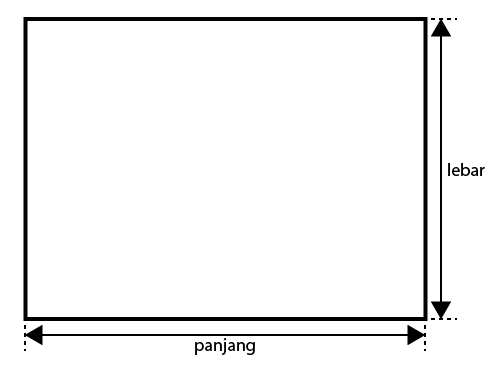
\includegraphics[scale=0.4]{model_ruangan}
	\caption[Pemodelan ruangan]{Pemodelan ruangan} 
	\label{fig:model_ruangan}
\end{figure}

%Dengan diketahuinya spesifikasi ruangan, maka akan diketahui daerah yang harus dicakup oleh kamera-kamera CCTV. Kamera-kamera CCTV akan ditempatkan dengan sedemian rupa sehingga seluruh daerah dapat tercakup. Untuk menyatakan posisi penempatan kamera CCTV, pemodelan masalah juga menggunakan sistem koordinat kertesius sehingga posisi penempatan dapat dinyatakan dalam koordinat x dan y. Dengan demikian, posisi penempatan kamera CCTV dapat dipahami lebih mudah.

Ruangan akan dipecah menjadi matriks \textit{cell} di mana masing-masing \textit{cell} menunjukkan bagian daerah terkecil dalam ruangan seperti pada gambar~\ref{fig:model_ruangan_cell}.

\begin{figure}[h]
	\centering  
	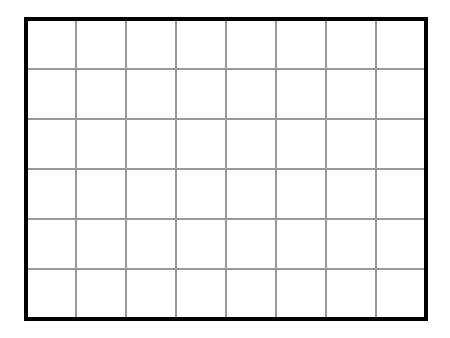
\includegraphics[scale=0.4]{model_ruangan_cell}
	\caption[Pemecahan ruangan menjadi matriks \textit{cell}]{Pemecahan ruangan menjadi matriks \textit{cell}} 
	\label{fig:model_ruangan_cell}
\end{figure}

Ukuran \textit{cell} dapat ditentukan berdasarkan ukuran terbesar yang dapat dimiliki oleh \textit{cell}. Didefinisikan variabel sebagai berikut:

\begin{equation}
	\begin{split}
		l &: \text{panjang ruangan}\\
		w &: \text{lebar ruangan}\\
		l_c &: \text{panjang \textit{cell}}\\
		w_c &: \text{lebar \textit{cell}}\\
		m &: \text{ukuran terbesar \textit{cell}}\\
	\end{split}
\end{equation}

Selanjutnya akan dicari ukuran matriks yang menghasilkan ukuran \textit{cell} yang tidak melebihi ukuran terbesar \textit{cell}:

\begin{equation}
	\begin{split}
		cols &: \text{jumlah kolom pada matriks \textit{cell}}\\
		rows &: \text{jumlah baris pada matriks \textit{cell}}\\
		cols &= \text{ceil}\left(\frac{l}{m}\right)\\
		rows &= \text{ceil}\left(\frac{w}{m}\right)\\
	\end{split}
\end{equation}

Setelah mendapatkan ukuran matriks, ukuran ruangan akan dibagi berdasarkan ukuran matriks sehingga didapatkan ukuran \textit{cell} yang tidak melebihi ukuran terbesar \textit{cell}:

\begin{equation}
	\begin{split}
		l_c &= \frac{l}{cols}\\
		w_c &= \frac{w}{rows}\\
	\end{split}
\end{equation}

\subsection{Kamera CCTV}
Kamera CCTV yang digunakan dalam masalah ini berbentuk sebagian lingkaran dalam bidang 2 dimensi. Kamera CCTV memiliki beragam parameter spesifikasi. Namun pada masalah ini, hanya terdapat 2 parameter spesifikasi yang digunakan, yaitu jarak pandang dan besar sudut pandang seperti pada gambar~\ref{fig:model_kamera}. Kedua parameter ini menentukan daerah yang dicakup oleh kamera CCTV. Jarak pandang menggunakan satuan ukuran sentimeter (cm) dan besar sudut pandang menggunakan satuan ukuran derajat (\(^\circ\)).

%Kamera CCTV yang beredar di pasaran memiliki spesifikasi yang sangat beragam. Dalam skripsi ini, jenis kamera CCTV yang digunakan dibatasi sehingga tidak bervariasi, yaitu hanya menggunakan 1 jenis kamera CCTV saja. Kamera CCTV sendiri memiliki berbagai parameter seperti jarak pandang, lebar sudut pandang, tingkat resolusi, dan parameter-parameter lainnya. Dalam masalah ini, terdapat 2 parameter yang digunakan, yaitu jarak pandang efektif dan lebar sudut pandang. Jarak pandang efektif merupakan jarak pandang terjauh kamera CCTV untuk mengenali suatu objek yang akan dipantau. Jarak pandang efektif dinyatakan dalam ukuran bersatuan sentimeter(cm) dan lebar sudut pandang dinyatakan dalam ukuran derajat. Pemodelan kamera CCTV dapat dipahami lebih lanjut pada gambar~\ref{fig:model_kamera}.

%Hingga saat ini, sudah terdapat banyak jenis kamera CCTV yang diproduksi. Setiap kamera CCTV tersebut memiliki spesifikasinya masing-masing. Dalam permasalahan ini, terdapat 2 spesifikasi kamera CCTV yang digunakan, yaitu jarak pandang efektif dan besar sudut pandang. Gambar~\ref{fig:model_kamera} memodelkan kamera CCTV dengan kedua spesifikasi tersebut. Jarak pandang efektif adalah jarak pandang terjauh kamera CCTV untuk mengenali objek yang akan dipantau. Besar sudut pandang menunjukkan lebar pantauan kamera CCTV. Dalam permasalahan ini, jenis kamera CCTV yang digunakan hanya berjumlah 1 buah.

\begin{figure}[h]
	\centering  
	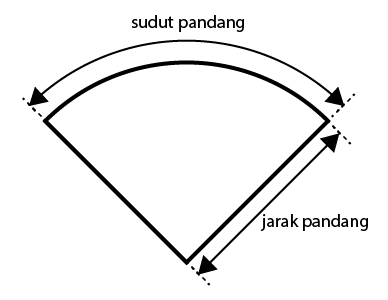
\includegraphics[scale=0.4]{model_kamera}
	\caption[Pemodelan kamera CCTV]{Pemodelan kamera CCTV} 
	\label{fig:model_kamera}
\end{figure}

Penempatan kamera CCTV dalam ruangan dinyatakan dalam 2 parameter, yaitu posisi penempatan dan arah pandang seperti pada gambar~\ref{fig:model_penempatan_kamera}. Posisi penempatan kamera CCTV dinyatakan dalam koordinat pada sistem koordinat kartesius 2 dimensi (\(x,y\)). Arah pandang menunjukkan arah yang dituju kamera CCTV. Arah pandang kamera CCTV dinyatakan dalam besar sudut derajat (\(^\circ\)) antara arah yang dituju dengan garis \(0^\circ\).

%\subsection{Penempatan Kamera CCTV}
%Setiap kamera CCTV dapat ditempatkan di mana saja selama berada di dalam ruangan. Penempatan kamera CCTV terdiri dari 2 komponen utama, yaitu posisi penempatan dan arah pandang. Posisi dan arah pandang akan mempengaruhi daerah cakupan kamera CCTV yang bersangkutan. Posisi penempatan dimodelkan dengan menggunakan sistem koordinat kartesius sehingga dapat dinyatakan dalam bentuk koordinat (x,y). Sumbu \(y\) pada sistem koordinat yang digunakan akan dibalik agar sesuai dengan lingkungan grafis pada layar komputer. Arah padang kamera CCTV dinyatakan sebagai besar sudut perpotongan antara garis tengah kamera CCTV dengan garis \(0^\circ\) yang dituliskan dalam satuan derajat. Dengan demikian, penempatan kamera CCTV terdiri atas posisi penempatan dan arah pandang yang dituju. Pemodelan penempatan kamera CCTV dapat dipahami lebih lanjut pada gambar~\ref{fig:model_penempatan_kamera}.

\begin{figure}[h]
	\centering  
	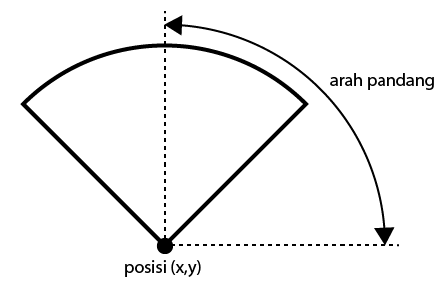
\includegraphics[scale=0.4]{model_penempatan_kamera}
	\caption[Penempatan kamera CCTV dalam ruangan]{Penempatan kamera CCTV dalam ruangan} 
	\label{fig:model_penempatan_kamera}
\end{figure}

\subsection{Cakupan Kamera CCTV}
Dengan pemecahan ruangan ke dalam matriks \textit{cell}, maka cakupan kamera CCTV dinyatakan dalam bentuk kumpulan cell. Contoh cakupan kamera CCTV dapat dilihat pada gambar~\ref{fig:cakupan_kamera_cctv}.

\begin{figure}[h]
	\centering  
	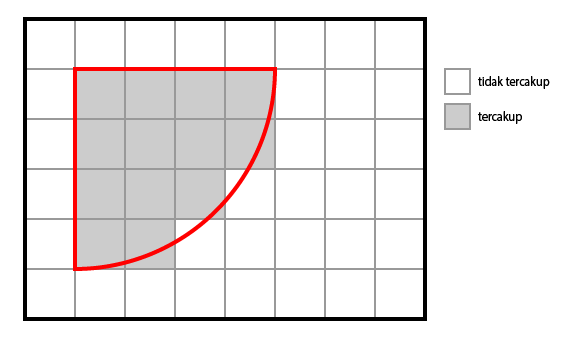
\includegraphics[scale=0.4]{daerah_cakupan_sesudah_grid_point}
	\caption[Cakupan kamera CCTV yang terdiri dari kumpulan \textit{cell}]{Cakupan kamera CCTV yang terdiri dari kumpulan \textit{cell}}
	\label{fig:cakupan_kamera_cctv}
\end{figure}

Setiap \textit{cell} memiliki titik tengah yang berada di tengah \textit{cell}. Titik tengah digunakan untuk menentukan ketercakupan \textit{cell} oleh suatu penempatan kamera CCTV. Untuk menentukan apakah suatu \textit{cell} dapat dicakup oleh suatu penempatan kamera CCTV, maka dilakukan 2 buah pengecekan. Pengecekan pertama dilakukan untuk memastikan bahwa jarak titik tengah \textit{cell} terhadap titik penempatan kamera CCTV lebih kecil atau sama dengan jarak pandang kamera CCTV. Untuk melakukannya, terlebih dahulu didefinisikan variabel sebagai berikut:
\begin{equation}
	\begin{split}
		(x_{cam},y_{cam}) &: \text{titik penempatan kamera CCTV}\\
		(x_{cell},y_{cell}) &: \text{titik tengah \textit{cell}}\\
		r &: \text{jarak pandang kamera CCTV}
	\end{split}
\end{equation}
Pengecekan pertama dinyatakan berhasil apabila memenuhi pernyataan berikut:
\begin{equation}
	\sqrt{(x_{cam} - x_{cell})^2 + (y_{cam} - y_{cell})^2} \leq r
\end{equation}
Pengecekan kedua dilakukan untuk memastikan bahwa titik tengah \textit{cell} berada di antara sudut pandang kamera CCTV. Untuk melakukannya, didefinisikan variabel dan fungsi sebagai berikut:
\begin{equation}
	\begin{split}
		\alpha &: \text{besar sudut pandang kamera CCTV}\\
		\beta &: \text{sudut arah pandang kamera CCTV}\\
		\text{norm}(\theta) &: \text{fungsi untuk menormalkan sudut sehingga } \theta \text{ berada dalam rentang }[0,2\pi)\\
		\text{atan2}(x,y) &: \text{fungsi untuk mendapatkan sudut rotasi titik } (x,y) \text{ terhadap titik O}\\
		\text{norm}(\theta) &=
		\left\{
			\begin{array}{ll}
				\text{norm}(\theta + 2\pi) & \text{jika } \theta < 0\\
				\text{norm}(\theta - 2\pi) & \text{jika } \theta \geq 2\pi\\
				\theta & \text{jika } \theta \geq 0 \text{ dan } \theta < 2\pi
			\end{array}
		\right.\\
		\text{atan2}(x,y) &=
		\left \{
			\begin{array}{ll}
				\arctan\left(\frac{y}{x}\right) & \text{jika } x>0\\
				\arctan\left(\frac{y}{x}\right)+\pi & \text{jika } x<0 \text{ dan } y\geq0\\
				\arctan\left(\frac{y}{x}\right)-\pi & \text{jika } x<0 \text{ dan } y<0\\
				+\frac{\pi}{2} & \text{jika } x=0 \text{ dan } y>0\\
				-\frac{\pi}{2} & \text{jika } x=0 \text{ dan } y<0\\
				\text{tak terdefinisi} & \text{jika } x=0 \text{ dan } y=0\\
			\end{array}
		\right.
	\end{split}
\end{equation}
Selanjutnya, akan dicari sudut pandang awal, sudut pandang akhir, dan sudut rotasi titik tengah \textit{cell} terhadap titik penempatan kamera CCTV:
\begin{equation}
	\begin{split}
		\alpha_{half} &: \text{setengah dari besar sudut pandang kamera CCTV}\\
		\beta_{start} &: \text{sudut pandang awal kamera CCTV}\\
		\beta_{end} &: \text{sudut pandang akhir kamera CCTV}\\
		\beta_{cell} &: \text{sudut rotasi titik tengah \textit{cell} terhadap titik penempatan kamera CCTV}\\
		\alpha_{half} &= \frac{\alpha}{2}\\
		\beta_{start} &= \text{norm}(\beta - \alpha_{half})\\
		\beta_{end} &= \text{norm}(\beta + \alpha_{half})\\
		\beta_{cell} &= \text{atan2}((y_{cell}-y_{cam}),(x_{cell}-x_{cam}))
	\end{split}
\end{equation}
Pengecekan kedua dibedakan berdasarkan sudut pandang awal dan sudut pandang akhir. Apabila sudut pandang awal lebih kecil daripada sudut pandang akhir, maka kedua pernyataan berikut harus dipenuhi agar pengecekan kedua dapat dinyatakan berhasil:
\begin{equation}
	\begin{split}
		\beta_{start} &< \beta_{cell}\\
		\beta_{cell} &< \beta_{end}\\
	\end{split}
\end{equation}
Apabila sudut pandang awal tidak lebih kecil daripada sudut pandang akhir, maka minimal satu dari kedua pernyataan berikut harus dipenuhi agar pengecekan kedua dapat dinyatakan berhasil:
\begin{equation}
	\begin{split}
		\beta_{start} &< \beta_{cell}\\
		\beta_{cell} &< \beta_{end}\\
	\end{split}
\end{equation}
Dengan memenuhi pengecekan pertama dan kedua, maka \textit{cell} dinyatakan tercakup oleh suatu penempatan kamera CCTV.

%Daerah cakupan kamera CCTV memiliki bentuk yang tidak sederhana sehingga menjadi sulit ketika akan diolah. Terdapat 3 kasus yang menjelaskan daerah cakupan dengan bentuk yang tidak sederhana ini, yaitu:
%\begin{enumerate}
%	\item Kasus ketika menghitung luas daerah yang tidak \textit{overlap} dan tidak \textit{out of bound}. Contoh kasus ini dapat dilihat pada gambar~\ref{fig:daerah_rumit} pada daerah yang dilabeli nomor 1.
%	\item Kasus ketika menghitung luas daerah \textit{overlap}. Contoh kasus ini dapat dilihat pada gambar~\ref{fig:daerah_rumit} pada daerah yang dilabeli nomor 2.
%	\item Kasus ketika menghitung luas daerah \textit{out of bound}. Contoh kasus ini dapat dilihat pada gambar~\ref{fig:daerah_rumit} pada daerah yang dilabeli nomor 3.
%\end{enumerate}
%
%\begin{figure}[h]
%	\centering  
%	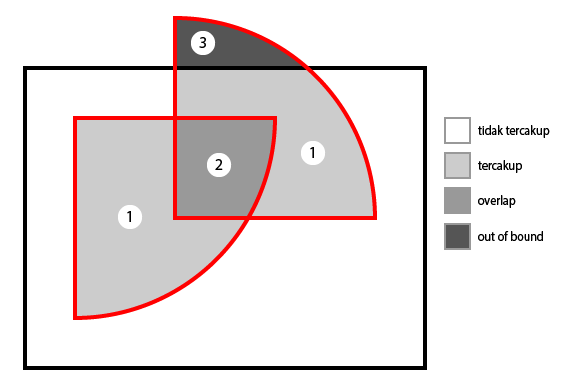
\includegraphics[scale=0.5]{daerah_rumit}
%	\caption[Contoh masalah yang memiliki kasus bentuk daerah tidak sederhana]{Contoh masalah yang memiliki kasus bentuk daerah tidak sederhana} 
%	\label{fig:daerah_rumit}
%\end{figure}
%
%Daerah-daerah dalam ketiga kasus tersebut dapat berbentuk tidak sederhana, sehingga sulit untuk diolah. Dengan adanya ketiga kasus ini, maka daerah cakupan perlu didefinisikan dan dimodelkan lebih lanjut agar kasus tersebut dapat dihindari. Ruangan dapat dimodelkan lebih lanjut sehingga berbentuk grid point seperti pada gambar~\ref{fig:model_ruangan_grid_point}. Grid point akan memecah ruangan ke dalam bagian-bagian yang lebih kecil yang disebut dengan cell.

%%\begin{figure}[h]
%%	\centering  
%%	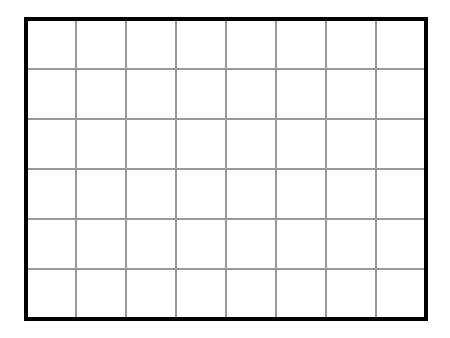
\includegraphics[scale=0.5]{model_ruangan_grid_point}
%%	\caption[Pemodelan ruangan dalam bentuk grid point]{Pemodelan ruangan dalam bentuk grid point} 
%%	\label{fig:model_ruangan_grid_point}
%%\end{figure}

%Cell tidak selalu berbentuk persegi, namun dapat berbentuk persegi panjang. Hal ini dikarenakan susunan cell-cell harus menghasilkan ukuran yang sama dengan ukuran ruangan. Untuk menentukan ukuran cell, ditentukan sebuah ukuran yang menyatakan ukuran terbesar yang dapat dimiliki cell. Ukuran ini akan digunakan untuk menentukan ukuran cell yang apabila disusun akan menghasilkan ukuran ruangan. Berikut ini merupakan rumus yang digunakan untuk mencari ukuran cell:

%\begin{equation*}
%	\begin{split}
%		\text{columns }&= \left\lceil\frac{\text{room width}}{\text{max cell size}}\right\rceil\\
%		\text{rows }&= \left\lceil\frac{\text{room length}}{\text{max cell size}}\right\rceil\\
%		\text{cell width }&= \frac{\text{room width}}{\text{columns}}\\
%		\text{cell length }&= \frac{\text{room length}}{\text{rows}}\\
%	\end{split}
%\end{equation*}

%Dengan rumus ini, akan didapatkan ukuran panjang dan ukuran lebar cell yang tidak melebihi ukuran terbesar cell. Apabila ukuran cell ini dikalikan dengan jumlah kolom dan jumlah baris grid point, maka akan didapatkan ukuran yang sama dengan ukuran ruangan.

%Setiap cell berfungsi merepresentasikan sebagian daerah dalam ruangan yang berupa satu kesatuan sehingga kasus bentuk daerah yang tidak sederhana dapat dihindari. Dengan pemodelan menggunakan grid point, maka daerah cakupan dari suatu kamera CCTV dapat dinyatakan dalam bentuk kumpulan cell. Gambar~\ref{fig:daerah_cakupan_sebelum_grid_point} dan gambar~\ref{fig:daerah_cakupan_sesudah_grid_point} menunjukkan perbandingan daerah cakupan kamera CCTV ketika sebelum dan sesudah dimodelkannya ruangan dalam bentuk grid point.

%\begin{figure}[h]
%	\centering  
%	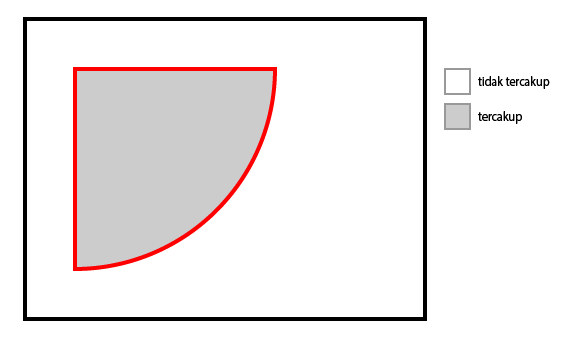
\includegraphics[scale=0.5]{daerah_cakupan_sebelum_grid_point}
%	\caption[Daerah cakupan sebelum pemodelan grid point]{Daerah cakupan sebelum pemodelan grid point}
%	\label{fig:daerah_cakupan_sebelum_grid_point}
%\end{figure}

%\begin{figure}[h]
%	\centering  
%	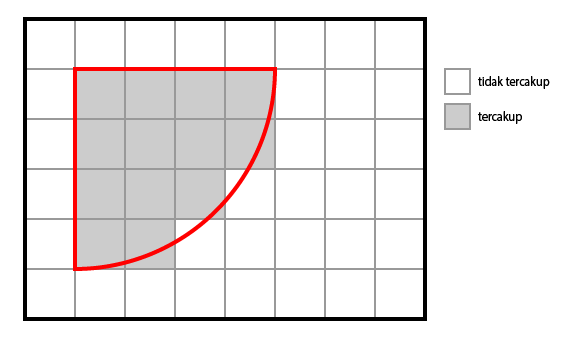
\includegraphics[scale=0.5]{daerah_cakupan_sesudah_grid_point}
%	\caption[Daerah cakupan sesudah pemodelan grid point]{Daerah cakupan sesudah pemodelan grid point}
%	\label{fig:daerah_cakupan_sesudah_grid_point}
%\end{figure}

%Untuk mencari kumpulan cell yang dicakup suatu penempatan kamera CCTV, maka setiap cell harus diperiksa apakah dapat tercakup oleh penempatan tersebut. Pada setiap cell akan ditentukan sebuah titik tengah yang berada di tengah-tengah cell. Titik tengah ini akan digunakan dalam pemeriksaan ketercakupan cell. Pemeriksaan terdiri dari pemeriksaan jarak cell dan pemeriksaan sudut rotasi cell. Jarak antara titik tengah cell dengan titik penempatan kamera CCTV harus lebih kecil daripada jarak pandang kamera CCTV. Sudut rotasi cell harus berada di antara sudut pandang kamera CCTV. Terdapat rumus yang digunakan untuk mendapatkan sudut rotasi ini, yaitu sebagai berikut:

%\begin{equation*}
%	atan2(x,y) =
%	\left \{
%  		\begin{array}{ll}
%  			\arctan(\frac{y}{x}) & \text{if } x>0\\
%  			\arctan(\frac{y}{x})+\pi & \text{if } x<0 \text{ and } y\geq0\\
%			\arctan(\frac{y}{x})-\pi & \text{if } x<0 \text{ and } y<0\\
%			+\frac{\pi}{2} & \text{if } x=0 \text{ and } y>0\\
%			-\frac{\pi}{2} & \text{if } x=0 \text{ and } y<0\\
%			\text{undefined} & \text{if } x=0 \text{ and } y=0\\
%  		\end{array}
%  	\right.
%\end{equation*}
%\begin{equation*}
%	\theta = atan2(y_{cam} - y_{cell}, x_{cell} - x_{cam})
%\end{equation*}

%Pada rumus tersebut, titik (\(x_{cell},y_{cell}\)) menunjukkan titik tengah cell dan titik (\(x_{cam},y_{cam}\)) menunjukkan titik penempatan kamera CCTV. Sudut rotasi cell (\(\theta\)) akan dibandingkan dengan sudut mulai dan sudut akhir dari sudut pandang kamera CCTV. Sudut rotasi harus berada di antara kedua sudut tersebut. Apabila kedua pemeriksaan tersebut berhasil dilalui, maka cell dinyatakan tercakup oleh kamera CCTV. Apabila sebaliknya, maka cell dinyatakan tidak tercakup oleh kamera CCTV. Dengan pemeriksaan ini, maka cakupan kamera CCTV dapat dicari dan dinyatakan dalam bentuk kumpulan cell.

%Cell-cell yang dicakup oleh kamera CCTV dapat dicari dengan memeriksa setiap cell pada ruangan. Pemeriksaan terdiri dari jarak cell dan sudut rotasi cell. Jarak titik tengah cell dengan posisi kamera CCTV harus lebih kecil daripada jarak pandang kamera CCTV. Sudut rotasi cell juga harus berada di antara sudut pandang kamera CCTV. Untuk mendapatkan sudut rotasi titik tengah cell terhadap posisi kamera, digunakan rumus berikut ini.
%\begin{equation*}
%	\theta = \tan^{-1}\left(\frac{y_2 - y_1}{x_2 - x_1}\right)
%\end{equation*}
%Sudut rotasi cell akan dibandingkan dengan sudut awal dan sudut akhir dari sudut pandang kamera CCTV. Apabila sudut rotasi berada di antara sudut awal dan sudut akhir, maka cell berada dalam sudut pandang kamera CCTV. Dengan memeriksa jarak dan sudut rotasi cell, cell-cell yang dicakup oleh kamera CCTV dapat ditemukan.
%\subsection{\textit{Overlap} dan \textit{Out of Bound}}
Perhitungan tingkat \textit{overlap} dan \textit{out of bound} dapat dilakukan dengan membandingkan jumlah \textit{cell}. \textit{Overlap cell} adalah \textit{cell} yang dicakup oleh lebih dari 1 kamera CCTV, sedangkan \textit{out of bound cell} adalah \textit{cell} di luar ruangan yang tercakup oleh kamera CCTV. Gambar~\ref{fig:daerah_overlap_out_of_bound} menggambarkan penempatan kamera CCTV yang menghasilkan \textit{overlap cell} dan \textit{out of bound cell}. Tingkat \textit{overlap} dan \textit{out of bound} dapat dihitung dengan mennjumlahkan semua \textit{cell} yang dicakup dari setiap kamera CCTV dan membaginya dengan jumlah \textit{cell} yang berada di dalam ruangan. Perhitungan tingkat \textit{overlap} dan \textit{out of bound} hanya dilakukan apabila seluruh \textit{cell} dalam ruangan telah tercakup oleh kamera CCTV.

\begin{figure}[h]
	\centering  
	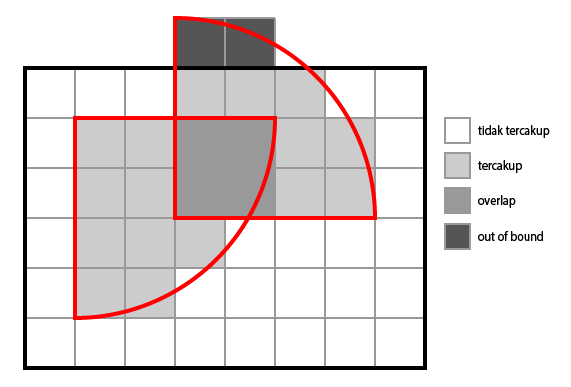
\includegraphics[scale=0.5]{daerah_overlap_out_of_bound}
	\caption[\textit{Overlap cell} dan \textit{out of bound cell}]{\textit{Overlap cell} dan \textit{out of bound cell}}
	\label{fig:daerah_overlap_out_of_bound}
\end{figure}

%Setiap cell dalam ruangan memiliki ukuran yang sama dengan cell-cell lainnya. Panjang harizontal dan vertikal dari cell tidak selalu berukuran sama sehingga cell dapat berbentuk persegi panjang. Penentuan ukuran cell merupakan bagian yang akan diteliti pada bagian eksperimen.


\section{Penyelesaian Masalah}
Dalam masalah ini, terdapat tujuan yang akan dicapai, yaitu mendapatkan penempatan-penempatan kamera CCTV yang dapat mencakup seluruh daerah pada ruangan. Kamera-kamera CCTV tentu dapat ditempatkan dimana saja hingga seluruh daerah pada ruangan tercakup sepenuhnya. Penempatan dengan cara ini tentu tidak efektif karena jumlah kamera CCTV tidak selalu berjumlah minimum sehingga diperlukan metode lainnya untuk menyelesaikan masalah ini. Salah satu cara yang digunakan untuk menyelesaikan masalah ini adalah dengan menggunakan teknik linear programming.

\subsection{Variabel Keputusan}
Pada awalnya ditentukan seluruh kemungkinan penempatan kamera CCTV sehingga setiap cell pada ruangan dicakup oleh minimal 1 kamera CCTV. Setiap penempatan kamera CCTV memiliki posisi dan arah pandang masing-masing. Dari seluruh kemungkinan ini akan dicari himpunan bagian yang dimana penempatan-penempatannya dapat mencakup seluruh daerah pada ruangan. Setiap kemungkinan penempatan memiliki 2 kemungkinan, yaitu diterapkan sebagai bagian dari solusi atau tidak. Dalam penyelesaian menggunakan teknik linear programming, setiap kemungkinan penempatan akan menjadi variabel keputusan. Variabel keputusan \(x_{ij\theta}\) akan merujuk pada penempatan kamera CCTV pada posisi \((i,j)\) dengan arah pandang \(\theta\). Karena setiap penempatan kamera CCTV memiliki 2 kemungkinan untuk diterapkan, maka setiap variabel keputusan dapat dinyatakan dengan nilai 0 atau 1. Apabila suatu variabel keputusan bernilai 1, maka penempatan kamera CCTV yang dirujuk akan diterapkan sebagai bagian dari solusi. Apabila benilai 0, maka penempatan kamera CCTV yang dirujuk tidak akan diterapkan. Karena variabel keputusan hanya bisa bernlai 0 dan 1 saja, masalah ini tidak diselesaikan menggunakan teknik linear programming biasa karena hasil dapat bernilai pecahan. Masalah ini perlu diselesaikan menggunakan teknik integer programming agar hasil dari setiap variabel keputusan hanya berupa bilangan bulat. Variabel keputusan dinyatakan dalam notasi berikut:

\begin{equation*}
	x_{ij\theta} =
	\left \{
  		\begin{tabular}{cl}
  			1 & jika kamera CCTV ditempatkan pada posisi $(i,j)$\\
  			  & dengan arah pandang $\theta$\\
  			  &  \\
  			0 & jika kamera CCTV tidak ditempatkan
  		\end{tabular}
  	\right.
\end{equation*}

\subsection{Fungsi Tujuan}
Solusi yang diharapkan dari masalah ini adalah mendapatkan penempatan-penempatan kamera CCTV yang paling minimum untuk mencakup seluruh daerah dalam ruangan. Dengan semakin sedikitnya penempatan-penempatan kamera CCTV yang digunakan, tingkat overlap dan out of bound juga akan semakin kecil. Sebelumnya telah diketahui bahwa setiap variabel keputusan hanya bisa bernilai 0 atau 1 saja. Jumlah penempatan kamera CCTV pun dapat dicari dengan menjumlahkan seluruh variabel keputusan. Fungsi tujuan dalam linear programming dapat dinyatakan sebagai jumlah penempatan kamera CCTV akan diminimumkan. Fungsi tujuan dituliskan dalam notasi berikut:

\begin{equation*}
	\textit{min }z = \sum_{\theta=0}^{s_{\theta}-1} \sum_{i=0}^{s_i-1} \sum_{j=0}^{s_j-1} x_{ij\theta}
\end{equation*}

\subsection{Batasan}
Selain mencari jumlah kamera CCTV yang minimal, seluruh daerah pada ruangan harus tercakup sepenuhnya. Berdasarkan pemodelan, ruangan dimodelkan dalam bentuk grid point sehingga daerah pada ruangan dimodelkan dalam bentuk cell. Agar seluruh daerah pada ruangan tercakup sepenuhnya, maka setiap cell harus dicakup oleh minimal 1 kamera CCTV. Terdapat sebuah fungsi biner yang digunakan untuk mengetahui apakah suatu penempatan kamera CCTV dapat mencakup suatu cell. Fungsi biner ini akan menghasilkan nilai 1 apabila suatu penempatan kamera CCTV dapat mencakup suatu cell. Apabila sebaliknya, maka fungsi biner ini akan menghasilkan nilai 0. Fungsi tersebut ditulis sebagai berikut:

\begin{equation*}
	cov(i,j,\theta,p,q) =
	\left \{
		\begin{tabular}{cl}
			1 & jika kamera CCTV pada posisi $(i,j)$ dengan arah pandang $\theta$\\
  			  & dapat mencakup cell $(p,q)$\\
  			  & \\
  			0 & jika sebaliknya
		\end{tabular}
	\right.
\end{equation*}

Dalam bentuk linear programming akan ditambahkan batasan yang menyatakan bahwa setiap cell harus dicakup oleh minimal 1 penempatan kamera CCTV. Fungsi biner sebelumnya akan digunakan untuk menyatakan hubungan ketercakupan cell dengan penempatan kamera CCTV. Batasan tersebut ditulis sebagai berikut:

\begin{equation*}
	\begin{split}
		& \sum_{\theta=0}^{s_{\theta}-1} \sum_{i=0}^{s_i-1} \sum_{j=0}^{s_j-1} x_{i,j,\theta} \times cov(i,j,\theta,p,q) \geq 1\\
		& 0 \leq p \leq (s_p - 1), 0 \leq q \leq (s_q - 1)
	\end{split}
\end{equation*}

\subsection{Bentuk Masalah Linear Programming}
Masalah yang dibahas di dalam skripsi ini dapat diubah ke dalam bentuk yang dapat diselesaikan dengan teknik linear programming. Setiap penempatan kamera CCTV pada ruangan menjadi variabel-variabel keputusan yang menunjukkan apakah akan diterapkan sebagai solusi atau tidak. Fungsi tujuan berfungsi untuk menyatakan bahwa penempatan-penempatan kamera CCTV harus berjumlah minimum sehingga sesuai dengan solusi yang diharapkan. Selain mendapatkan jumlah penempatan kamera CCTV yang minimum, terdapat batasan-batasan yang menyatakan bahwa seluruh daerah pada ruangan juga harus tercakup sepenuhnya. Apabila digabungkan, maka bentuk masalah ini dalam bentuk linear programming adalah seperti berikut:

\begin{equation*}
	\begin{split}
		\textit{min } & z = \sum_{\theta=0}^{s_{\theta}-1} \sum_{i=0}^{s_i-1} \sum_{j=0}^{s_j-1} x_{ij\theta}\\
		\textit{s.t. } & \sum_{\theta=0}^{s_{\theta}-1} \sum_{i=0}^{s_i-1} \sum_{j=0}^{s_j-1} x_{i,j,\theta} \times cov(i,j,\theta,p,q) \geq 1\\
		& 0 \leq p \leq (s_p - 1), 0 \leq q \leq (s_q - 1)\\
		& x_{ij\theta} \in \{0,1\}
	\end{split}
\end{equation*}

\section{Analisis Kebutuhan Perangkat Lunak}
Pada subbab ini, akan dijelaskan aksi-aksi yang dapat dilakukan pengguna terhadap perangkat lunak melalui diagram \textit{use case} dan skenario-skenario. Selain penjelasan aksi-aksi, terdapat juga diagram kelas sederhana yang akan dikembangkan lebih lanjut pada tahap perancangan perangkat lunak. 
%Pada subbab ini akan dijelaskan deskripsi dari perangkat lunak yang akan dibangun. Perangkat lunak yang dibangun akan disesuaikan dengan pemodelan masalah yang telah dibahas sebelumnya. Perangkat lunak akan menggunakan fitur tampilan antarmuka grafis untuk memudahkan interaksi pengguna dengan perangkat lunak. Perangkat lunak akan mengsimulasikan masalah penempatan kamera CCTV dengan masukan yang dimasukkan oleh pengguna. Hasil dari masukan pengguna akan diolah oleh perangkat lunak dan hasilnya akan ditampilkan. Rancangan perangkat lunak yang terdiri dari diagram use case, diagram kelas, masukan, dan keluaran akan dibahas pada bagian ini.

\subsection{Diagram \textit{Use Case}}
Dalam perangkat lunak yang dibangun, hanya terdapat 1 jenis pengguna. Diagram \textit{use case} pada gambar~\ref{fig:use_case_diagram} menunjukkan aktor dan aksi-aksi yang dapat dilakukannya.
\begin{figure}[h]
	\centering  
	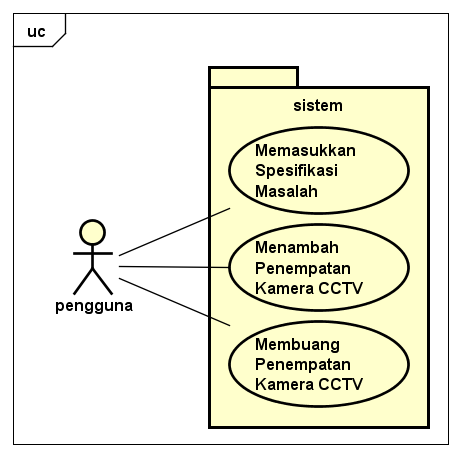
\includegraphics[scale=0.72]{use_case_diagram}
	\caption[Diagram \textit{use case}]{Diagram \textit{use case}}
	\label{fig:use_case_diagram}
\end{figure}

Berikut ini skenario dari setiap aksi pada diagram \textit{use case}:
\begin{itemize}
	\item Skenario: \textbf{Memasukkan Spesifikasi Masalah}
	\begin{itemize}
		\item Aktor: Pengguna
		\item Langkah:
		\begin{enumerate}
			\item Aktor memasukkan spesifikasi masalah yang terdiri dari ukuran ruangan dan spesifikasi kamera CCTV dan dilanjutkan dengan menekan tombol ''\textit{submit}''.
			\item Sistem menampilkan tampilan simulasi penempatan kamera CCTV.
		\end{enumerate}
	\end{itemize}
	\item Skenario: \textbf{Menambah Penempatan Kamera CCTV}
	\begin{itemize}
		\item Aktor: Pengguna
		\item Langkah:
		\begin{enumerate}
			\item Aktor memilih posisi penempatan kamera CCTV dan mengisi sudut arah pandang penempatan kamera CCTV dan dilanjutkan dengan menekan tombol ''\textit{add camera}''.
			\item Sistem menambahkan penempatan ke dalam simulasi dan memperbaharui tampilan simulasi.
		\end{enumerate}
	\end{itemize}
%	\item Skenario: \textbf{Menyelesaikan Masalah Secara Otomatis}
%	\begin{itemize}
%		\item Aktor: Pengguna
%		\item Langkah:
%		\begin{enumerate}
%			\item Aktor menekan tombol ''\textit{auto solve}''.
%			\item Sistem menganalisa kondisi masalah dan mencari penempatan-penempatan kamera CCTV.
%			\item Sistem menambahkan penempatan-penempatan kamera CCTV ke dalam simulasi secara otomatis.
%			\item Sistem memperbaharui visualisasi penempatan kamera CCTV.
%			\item Sistem memperbaharui panel informasi.
%		\end{enumerate}
%	\end{itemize}
	\item Skenario: \textbf{Membuang Penempatan Kamera CCTV}
	\begin{itemize}
		\item Aktor: Pengguna
		\item Langkah:
		\begin{enumerate}
			\item Aktor memilih penempatan kamera CCTV yang akan dibuang dan menekan tombol ''\textit{remove}''.
			\item Sistem membuang penempatan dari simulasi dan memperbaharui tampilan simulasi.
		\end{enumerate}
	\end{itemize}
\end{itemize}

\subsection{Diagram Kelas}
Pada bagian ini terdapat diagram kelas sederhana yang menunjukkan kelas-kelas yang akan digunakan untuk merancang perangkat lunak. Diagram kelas sederhana dapat dilihat pada gambar~\ref{fig:class_diagram_basic}.

\begin{figure}[h]
	\centering  
	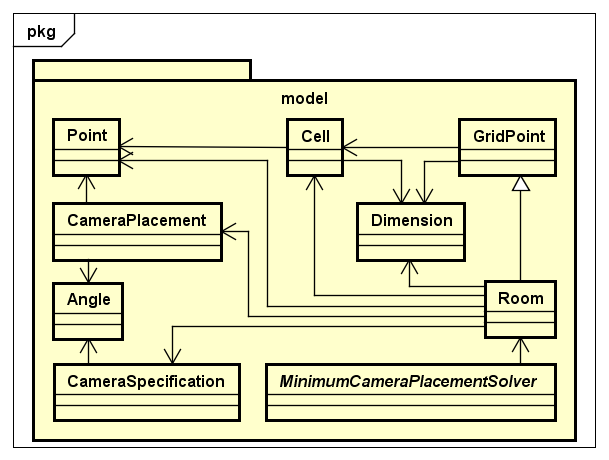
\includegraphics[scale=0.6]{class_diagram_basic}
	\caption[Diagram kelas sederhana]{Diagram kelas sederhana}
	\label{fig:class_diagram_basic}
\end{figure}